% Options for packages loaded elsewhere
\PassOptionsToPackage{unicode}{hyperref}
\PassOptionsToPackage{hyphens}{url}
%
\documentclass[
]{book}
\usepackage{lmodern}
\usepackage{amssymb,amsmath}
\usepackage{ifxetex,ifluatex}
\ifnum 0\ifxetex 1\fi\ifluatex 1\fi=0 % if pdftex
  \usepackage[T1]{fontenc}
  \usepackage[utf8]{inputenc}
  \usepackage{textcomp} % provide euro and other symbols
\else % if luatex or xetex
  \usepackage{unicode-math}
  \defaultfontfeatures{Scale=MatchLowercase}
  \defaultfontfeatures[\rmfamily]{Ligatures=TeX,Scale=1}
\fi
% Use upquote if available, for straight quotes in verbatim environments
\IfFileExists{upquote.sty}{\usepackage{upquote}}{}
\IfFileExists{microtype.sty}{% use microtype if available
  \usepackage[]{microtype}
  \UseMicrotypeSet[protrusion]{basicmath} % disable protrusion for tt fonts
}{}
\makeatletter
\@ifundefined{KOMAClassName}{% if non-KOMA class
  \IfFileExists{parskip.sty}{%
    \usepackage{parskip}
  }{% else
    \setlength{\parindent}{0pt}
    \setlength{\parskip}{6pt plus 2pt minus 1pt}}
}{% if KOMA class
  \KOMAoptions{parskip=half}}
\makeatother
\usepackage{xcolor}
\IfFileExists{xurl.sty}{\usepackage{xurl}}{} % add URL line breaks if available
\IfFileExists{bookmark.sty}{\usepackage{bookmark}}{\usepackage{hyperref}}
\hypersetup{
  pdftitle={MA22004 Course Design Plan},
  pdfauthor={Dr Eric Hall (ehall001@dundee.ac.uk)},
  hidelinks,
  pdfcreator={LaTeX via pandoc}}
\urlstyle{same} % disable monospaced font for URLs
\usepackage{color}
\usepackage{fancyvrb}
\newcommand{\VerbBar}{|}
\newcommand{\VERB}{\Verb[commandchars=\\\{\}]}
\DefineVerbatimEnvironment{Highlighting}{Verbatim}{commandchars=\\\{\}}
% Add ',fontsize=\small' for more characters per line
\usepackage{framed}
\definecolor{shadecolor}{RGB}{248,248,248}
\newenvironment{Shaded}{\begin{snugshade}}{\end{snugshade}}
\newcommand{\AlertTok}[1]{\textcolor[rgb]{0.94,0.16,0.16}{#1}}
\newcommand{\AnnotationTok}[1]{\textcolor[rgb]{0.56,0.35,0.01}{\textbf{\textit{#1}}}}
\newcommand{\AttributeTok}[1]{\textcolor[rgb]{0.77,0.63,0.00}{#1}}
\newcommand{\BaseNTok}[1]{\textcolor[rgb]{0.00,0.00,0.81}{#1}}
\newcommand{\BuiltInTok}[1]{#1}
\newcommand{\CharTok}[1]{\textcolor[rgb]{0.31,0.60,0.02}{#1}}
\newcommand{\CommentTok}[1]{\textcolor[rgb]{0.56,0.35,0.01}{\textit{#1}}}
\newcommand{\CommentVarTok}[1]{\textcolor[rgb]{0.56,0.35,0.01}{\textbf{\textit{#1}}}}
\newcommand{\ConstantTok}[1]{\textcolor[rgb]{0.00,0.00,0.00}{#1}}
\newcommand{\ControlFlowTok}[1]{\textcolor[rgb]{0.13,0.29,0.53}{\textbf{#1}}}
\newcommand{\DataTypeTok}[1]{\textcolor[rgb]{0.13,0.29,0.53}{#1}}
\newcommand{\DecValTok}[1]{\textcolor[rgb]{0.00,0.00,0.81}{#1}}
\newcommand{\DocumentationTok}[1]{\textcolor[rgb]{0.56,0.35,0.01}{\textbf{\textit{#1}}}}
\newcommand{\ErrorTok}[1]{\textcolor[rgb]{0.64,0.00,0.00}{\textbf{#1}}}
\newcommand{\ExtensionTok}[1]{#1}
\newcommand{\FloatTok}[1]{\textcolor[rgb]{0.00,0.00,0.81}{#1}}
\newcommand{\FunctionTok}[1]{\textcolor[rgb]{0.00,0.00,0.00}{#1}}
\newcommand{\ImportTok}[1]{#1}
\newcommand{\InformationTok}[1]{\textcolor[rgb]{0.56,0.35,0.01}{\textbf{\textit{#1}}}}
\newcommand{\KeywordTok}[1]{\textcolor[rgb]{0.13,0.29,0.53}{\textbf{#1}}}
\newcommand{\NormalTok}[1]{#1}
\newcommand{\OperatorTok}[1]{\textcolor[rgb]{0.81,0.36,0.00}{\textbf{#1}}}
\newcommand{\OtherTok}[1]{\textcolor[rgb]{0.56,0.35,0.01}{#1}}
\newcommand{\PreprocessorTok}[1]{\textcolor[rgb]{0.56,0.35,0.01}{\textit{#1}}}
\newcommand{\RegionMarkerTok}[1]{#1}
\newcommand{\SpecialCharTok}[1]{\textcolor[rgb]{0.00,0.00,0.00}{#1}}
\newcommand{\SpecialStringTok}[1]{\textcolor[rgb]{0.31,0.60,0.02}{#1}}
\newcommand{\StringTok}[1]{\textcolor[rgb]{0.31,0.60,0.02}{#1}}
\newcommand{\VariableTok}[1]{\textcolor[rgb]{0.00,0.00,0.00}{#1}}
\newcommand{\VerbatimStringTok}[1]{\textcolor[rgb]{0.31,0.60,0.02}{#1}}
\newcommand{\WarningTok}[1]{\textcolor[rgb]{0.56,0.35,0.01}{\textbf{\textit{#1}}}}
\usepackage{longtable,booktabs}
% Correct order of tables after \paragraph or \subparagraph
\usepackage{etoolbox}
\makeatletter
\patchcmd\longtable{\par}{\if@noskipsec\mbox{}\fi\par}{}{}
\makeatother
% Allow footnotes in longtable head/foot
\IfFileExists{footnotehyper.sty}{\usepackage{footnotehyper}}{\usepackage{footnote}}
\makesavenoteenv{longtable}
\usepackage{graphicx}
\makeatletter
\def\maxwidth{\ifdim\Gin@nat@width>\linewidth\linewidth\else\Gin@nat@width\fi}
\def\maxheight{\ifdim\Gin@nat@height>\textheight\textheight\else\Gin@nat@height\fi}
\makeatother
% Scale images if necessary, so that they will not overflow the page
% margins by default, and it is still possible to overwrite the defaults
% using explicit options in \includegraphics[width, height, ...]{}
\setkeys{Gin}{width=\maxwidth,height=\maxheight,keepaspectratio}
% Set default figure placement to htbp
\makeatletter
\def\fps@figure{htbp}
\makeatother
\setlength{\emergencystretch}{3em} % prevent overfull lines
\providecommand{\tightlist}{%
  \setlength{\itemsep}{0pt}\setlength{\parskip}{0pt}}
\setcounter{secnumdepth}{5}
\usepackage[]{natbib}
\bibliographystyle{plainnat}

\title{MA22004 Course Design Plan}
\author{Dr Eric Hall \href{mailto:ehall001@dundee.ac.uk}{(ehall001@dundee.ac.uk)}}
\date{2020-07-22}

\begin{document}
\maketitle

{
\setcounter{tocdepth}{1}
\tableofcontents
}
\hypertarget{learning}{%
\chapter{Teaching-Learning Activities}\label{learning}}

\begin{quote}
\emph{Wir shaffen das.}
\end{quote}

\emph{Summary:} MA22004 will run for 11 weeks (20 SCQF/10 ECTS) requiring approximately 200 hours student effort (or 17.5 hours per week less the examination time). On an average week there will be seven planned teaching and learning activities, detailed below. These include 1 seminar (1 h duration, \textbf{timetabled}, \textbf{online}), 1 workshop (1 hour duration, \textbf{timetabled}, \textbf{face-to-face}), and 1 lab (approx. variable duration, \textbf{online, asynchronous}). The expectation will be that students access and engage with the lecture notes and curated digital content before participating in the seminar.

\hypertarget{seminar-reading}{%
\section{Seminar Reading}\label{seminar-reading}}

\begin{quote}
This activity contains an \protect\hyperlink{engagement}{engagement} measure.
\end{quote}

\begin{longtable}[]{@{}lllll@{}}
\toprule
\endhead
\emph{Read Watch Listen} & \emph{3 hours} & \emph{1 student} & \emph{Tutor is not available} & \emph{Online}\tabularnewline
\bottomrule
\end{longtable}

Read lecture notes.

\begin{longtable}[]{@{}lllll@{}}
\toprule
\endhead
\emph{Collaborate} & \emph{1 hour} & \emph{6 students} & \emph{Tutor is not available} & \emph{Online}\tabularnewline
\bottomrule
\end{longtable}

(Pre Seminar) Comment on lecture notes through Persuall (measure
engagement by fixed number of questions/answers asked).

\begin{longtable}[]{@{}lllll@{}}
\toprule
\endhead
\emph{Investigate} & \emph{1 hour} & \emph{1 student} & \emph{Tutor is not available} & \emph{Online}\tabularnewline
\bottomrule
\end{longtable}

(Post Seminar) Understand connections between material by exploring
comments and questions and through reflection.

\hypertarget{preparation-seminar-investigation}{%
\section{Preparation: Seminar Investigation}\label{preparation-seminar-investigation}}

\begin{longtable}[]{@{}lllll@{}}
\toprule
\endhead
\emph{Investigate} & \emph{1 hour} & \emph{1 student} & \emph{Tutor is not available} & \emph{Online}\tabularnewline
\bottomrule
\end{longtable}

Supplementary online material (curated content).

\hypertarget{seminar}{%
\section{Seminar}\label{seminar}}

\begin{quote}
This activity contains both \protect\hyperlink{engagement}{engagement} and \protect\hyperlink{assessment}{assessment} measures.
\end{quote}

\begin{longtable}[]{@{}lllll@{}}
\toprule
\endhead
\emph{Produce} & \emph{10 minutes} & \emph{1 student} & \emph{Tutor is available} & \emph{Online}\tabularnewline
\bottomrule
\end{longtable}

Seminar quiz (measure attainment based on quiz grade).

\begin{longtable}[]{@{}lllll@{}}
\toprule
\endhead
\emph{Discuss} & \emph{40 minutes} & \emph{60 students} & \emph{Tutor is available} & \emph{Online}\tabularnewline
\bottomrule
\end{longtable}

Review key points of material with appropriate polling (measure
engagement by participation in polling and discussion).

\begin{longtable}[]{@{}lllll@{}}
\toprule
\endhead
\emph{Practice} & \emph{10 minutes} & \emph{6 students} & \emph{Tutor is available} & \emph{Online}\tabularnewline
\bottomrule
\end{longtable}

Student presentations: either a lab presentation or solutions to the seminar quiz. Students who are not presenting a lab presentation will be expected to provide the presenting group with feedback (through blackboard).

\hypertarget{computer-lab}{%
\section{Computer lab}\label{computer-lab}}

\begin{quote}
This activity contains both \protect\hyperlink{engagement}{engagement} and \protect\hyperlink{assessment}{assessment} measures.
\end{quote}

\begin{longtable}[]{@{}lllll@{}}
\toprule
\endhead
\emph{Read Watch Listen} & \emph{1 hour and 30 minutes} & \emph{1 student} & \emph{Tutor is not available} & \emph{Online}\tabularnewline
\bottomrule
\end{longtable}

Read instructions and examples.

\begin{longtable}[]{@{}lllll@{}}
\toprule
\endhead
\emph{Practice} & \emph{2 hours} & \emph{1 student} & \emph{Tutor is not available} & \emph{Online}\tabularnewline
\bottomrule
\end{longtable}

Practice coding and respond to simple interactive elements that deliver
instant feedback (measure engagement by responding to interactive
elements).

\begin{longtable}[]{@{}lllll@{}}
\toprule
\endhead
\emph{Produce} & \emph{2 hours} & \emph{1 student} & \emph{Tutor is not available} & \emph{Online}\tabularnewline
\bottomrule
\end{longtable}

Answer review questions and submit for evaluation (measure attainment
based on answers to review questions).

\hypertarget{preparation-workshop}{%
\section{Preparation: Workshop}\label{preparation-workshop}}

\begin{longtable}[]{@{}lllll@{}}
\toprule
\endhead
\emph{Practice} & \emph{2 hours} & \emph{1 student} & \emph{Tutor is not available} & \emph{Online}\tabularnewline
\bottomrule
\end{longtable}

Attempt workshop problems.

\hypertarget{workshop-face-to-face}{%
\section{Workshop (Face-to-face)}\label{workshop-face-to-face}}

\begin{longtable}[]{@{}lllll@{}}
\toprule
\endhead
\emph{Collaborate} & \emph{1 hour} & \emph{6 students} & \emph{Tutor is available} & \emph{F2F}\tabularnewline
\bottomrule
\end{longtable}

Students discuss problems together in small groups. \emph{This could be done
using break-out rooms if face-to-face meeting not possible.}

\hypertarget{office-hours}{%
\section{Office Hours}\label{office-hours}}

\begin{longtable}[]{@{}lllll@{}}
\toprule
\endhead
\emph{Discuss} & \emph{2 hours} & \emph{6 students} & \emph{Tutor is available} & \emph{Online}\tabularnewline
\bottomrule
\end{longtable}

Instructor available to answer questions about lab/reading. Typically
this will not be one-on-one but small group meetings.

\hypertarget{representations-of-the-learning-experience}{%
\section*{Representations of the learning experience}\label{representations-of-the-learning-experience}}
\addcontentsline{toc}{section}{Representations of the learning experience}

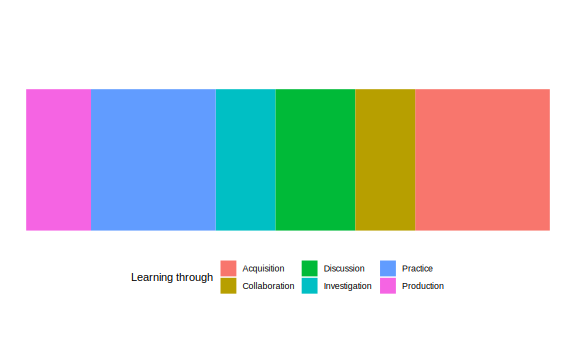
\includegraphics{design-notes_files/figure-latex/table-learning-1.pdf}

\begin{tabular}{l|r|r}
\hline
Learning through & Minutes & Percent\\
\hline
Acquisition & 270 & 26\\
\hline
Investigation & 120 & 11\\
\hline
Discussion & 160 & 15\\
\hline
Practice & 250 & 24\\
\hline
Collaboration & 120 & 11\\
\hline
Production & 130 & 12\\
\hline
\end{tabular}

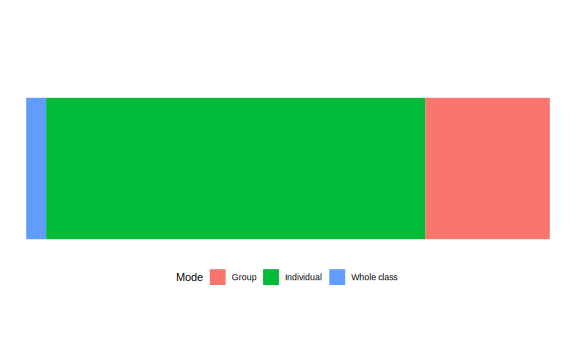
\includegraphics{design-notes_files/figure-latex/table-group-1.pdf}

\begin{tabular}{l|r|r}
\hline
Mode & Minutes & Percent\\
\hline
Whole class & 40 & 4\\
\hline
Group & 250 & 24\\
\hline
Individual & 760 & 72\\
\hline
\end{tabular}

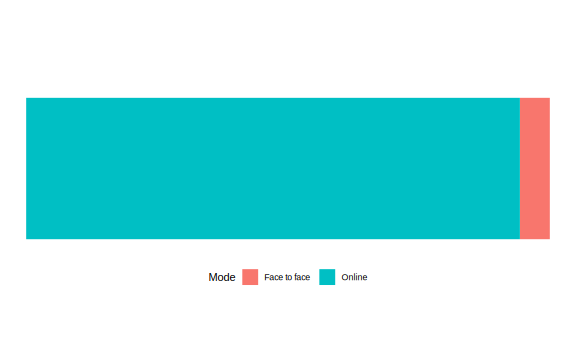
\includegraphics{design-notes_files/figure-latex/table-f2f-1.pdf}

\begin{tabular}{l|r|r}
\hline
Mode & Minutes & Percent\\
\hline
Face to face & 60 & 6\\
\hline
Online & 990 & 94\\
\hline
\end{tabular}

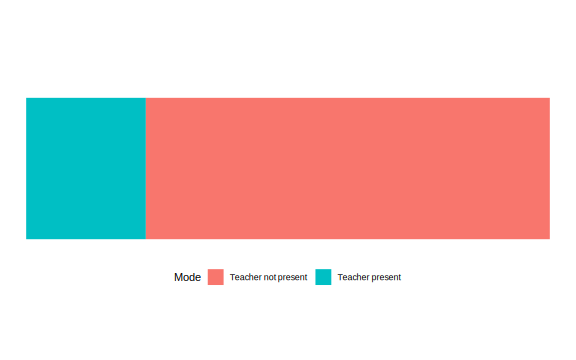
\includegraphics{design-notes_files/figure-latex/table-present-1.pdf}

\begin{tabular}{l|r|r}
\hline
Mode & Minutes & Percent\\
\hline
Teacher present & 240 & 23\\
\hline
Teacher not present & 810 & 77\\
\hline
\end{tabular}

\hypertarget{engagement}{%
\chapter{Engagement and Attainment}\label{engagement}}

\begin{quote}
The active learning categorization for each activity is identified in \protect\hyperlink{learning}{§ Learning}.
\end{quote}

\hypertarget{engagement-plan}{%
\section{Engagement Plan}\label{engagement-plan}}

There are several points that can be measured to assess engagement, including:

\begin{itemize}
\tightlist
\item
  \textbf{Seminar Reading} Students will be presented with a new collection of notes weekly using \href{https://perusall.com/}{Perusall}. Students will be responsible for reading notes posting both questions/comments and responses (collaborative annotation). Student engagement will be tracked in Perusall through quality of discourse.
\item
  \textbf{Seminar} During seminars, students will be presented with \emph{live polls}, using either \href{https://www.mentimeter.com/}{Mentimeter} or \href{https://itempool.com/}{Itempool}, to encourage reflection and discussion. Student engagement will be assessed through participation.
\item
  \textbf{Seminar} During seminars, students will take turns \emph{presenting} a lab report or quiz solutions with their workshop groups. This will encourage students to challenge their peer's analysis. Student engagement will be assessed through participation.
\item
  \textbf{Computer Lab} Students will be required to \emph{respond} to questions that will be computer-graded in interactive computer labs. Student engagement will be assessed through quality of responses.
\end{itemize}

\hypertarget{attainment-plan}{%
\section{Attainment Plan}\label{attainment-plan}}

Student attainment will be assessed continuously through the evaluation of student produced materials and presentations. These items include:
+ lab reports,
+ lab presentation (group),
+ two midterm examinations (computer graded).
The grades of these continuous assessment will offer opportunities for intervention and students will receive
The final examination will provide a comprehensive assessment of the whole course.

\hypertarget{assessment}{%
\chapter{Assessment}\label{assessment}}

The module assessment will be weighted:

\begin{tabular}{l|l}
\hline
Assessment & Weight\\
\hline
Assignments & 20\%\\
\hline
Midterm Exam 1 & 20\%\\
\hline
Midterm Exam 2 & 20\%\\
\hline
Final Exam & 40\%\\
\hline
\end{tabular}

Note: This is a modification from the previous split (60\% degree exam, 20\% two
class tests, and 20\% coursework). As the students will not be given a revision period, the Final Exam will need to be less cumulative in scope and therefore additional weight will be placed on the Midterm Exams.

\hypertarget{examinations}{%
\section{Examinations}\label{examinations}}

The \textbf{Midterm Exams} will be computer-assessed and will be 1 hour in scope (compared to the 2 hour Final Exam). These will likely be held in week 4 and week 8.

The \textbf{Final Exam} will be a 2 hour hand-written exam. Students will be given one additional hour to scan, code, and upload their manuscripts using \href{https://www.gradescope.com/}{Gradescope}. This process will be thoroughly discussed and practiced by the students with a dummy exam in advance of a real submission. The Final Exam will be given in the last week of term (i.e., during week 11).

\hypertarget{assignments}{%
\section{Assignments}\label{assignments}}

The assessed coursework will include 6 lab reports and 1 lab report presentation (group work).

\hypertarget{needs}{%
\chapter{NEEDS}\label{needs}}

\hypertarget{digital-needs}{%
\section*{Digital needs}\label{digital-needs}}
\addcontentsline{toc}{section}{Digital needs}

\begin{enumerate}
\def\labelenumi{\arabic{enumi}.}
\tightlist
\item
  bringing computer lab into cloud: semester subsription to \href{https://rstudio.cloud/}{RStudio Cloud}\footnote{A better long-term solution would be to run \texttt{RStudio\ Server\ Pro} and \texttt{RStudio\ Connect} on in-house server running, licenses are available for \href{https://rstudio.com/pricing/academic-pricing/}{free} for teaching purposes.} (approx. 1000 USD)
\item
  polling: \href{https://www.mentimeter.com/}{mentimeter} or \href{https://itempool.com/}{itempool}
\end{enumerate}

\hypertarget{hardware-needs}{%
\section*{Hardware needs}\label{hardware-needs}}
\addcontentsline{toc}{section}{Hardware needs}

\begin{enumerate}
\def\labelenumi{\arabic{enumi}.}
\tightlist
\item
  Better microphone
\item
  Tablet with stylus
\end{enumerate}

\hypertarget{rmarkdown-example}{%
\chapter*{Rmarkdown Example}\label{rmarkdown-example}}
\addcontentsline{toc}{chapter}{Rmarkdown Example}

\hypertarget{math}{%
\section*{Math}\label{math}}
\addcontentsline{toc}{section}{Math}

Here is an example page containing math markdown.

\begin{Shaded}
\begin{Highlighting}[]
\NormalTok{We can use inline math, }\SpecialStringTok{$f\_X$}\NormalTok{, }\SpecialStringTok{$f\_Y$}\NormalTok{, and }\SpecialStringTok{$f\_\{X,Y\}$}\NormalTok{, as well as display math, }
\SpecialStringTok{\textbackslash{}[}
\SpecialStringTok{  I(X;Y)}
\SpecialStringTok{  = }\SpecialCharTok{\textbackslash{}iint}\SpecialStringTok{\_\{}\SpecialCharTok{\textbackslash{}mathcal}\SpecialStringTok{\{X\} }\SpecialCharTok{\textbackslash{}otimes}\SpecialStringTok{ }\SpecialCharTok{\textbackslash{}mathcal}\SpecialStringTok{\{Y\}\}}
\SpecialStringTok{  }\SpecialCharTok{\textbackslash{}log\textbackslash{}left}\SpecialStringTok{( }\SpecialCharTok{\textbackslash{}frac}\SpecialStringTok{\{f\_\{X,Y\}(x,y)\}\{f\_\{X\}(x)f\_\{Y\}(y)\} }\SpecialCharTok{\textbackslash{}right}\SpecialStringTok{)}
\SpecialStringTok{  f\_\{X,Y\}(x,y) }\SpecialCharTok{\textbackslash{}mathrm}\SpecialStringTok{\{d\}y }\SpecialCharTok{\textbackslash{}mathrm}\SpecialStringTok{\{d\}x}\SpecialCharTok{\textbackslash{},}\SpecialStringTok{.}
\SpecialStringTok{\textbackslash{}]}
\end{Highlighting}
\end{Shaded}

to generate:

We can use inline math, \(f_X\), \(f_Y\), and \(f_{X,Y}\), as well as display math,
\[
  I(X;Y)
  = \iint_{\mathcal{X} \otimes \mathcal{Y}}
  \log\left( \frac{f_{X,Y}(x,y)}{f_{X}(x)f_{Y}(y)} \right)
  f_{X,Y}(x,y) \mathrm{d}y \mathrm{d}x\,.
\]

\hypertarget{plots}{%
\section*{Plots}\label{plots}}
\addcontentsline{toc}{section}{Plots}

\begin{Shaded}
\begin{Highlighting}[]
\NormalTok{x \textless{}{-}}\StringTok{ }\KeywordTok{seq}\NormalTok{(}\OperatorTok{{-}}\DecValTok{8}\NormalTok{, }\DecValTok{8}\NormalTok{, }\DataTypeTok{length=}\DecValTok{1000}\NormalTok{)}
\NormalTok{y0 \textless{}{-}}\StringTok{ }\KeywordTok{dnorm}\NormalTok{(x, }\DecValTok{{-}2}\NormalTok{, }\DecValTok{1}\NormalTok{)}
\NormalTok{y1 \textless{}{-}}\StringTok{ }\KeywordTok{dnorm}\NormalTok{(x, }\DecValTok{2}\NormalTok{, }\DecValTok{1}\NormalTok{)}
\NormalTok{df \textless{}{-}}\StringTok{ }\KeywordTok{tibble}\NormalTok{(x, y0, y1)}
\NormalTok{df \textless{}{-}}\StringTok{ }\KeywordTok{melt}\NormalTok{(df, }\DataTypeTok{id.var =} \StringTok{"x"}\NormalTok{, }\DataTypeTok{value.name =} \StringTok{"y"}\NormalTok{)}

\KeywordTok{ggplot}\NormalTok{(}\DataTypeTok{data =}\NormalTok{ df, }\KeywordTok{aes}\NormalTok{(}\DataTypeTok{x =}\NormalTok{ x, }\DataTypeTok{color =}\NormalTok{ variable)) }\OperatorTok{+}\StringTok{ }\KeywordTok{geom\_line}\NormalTok{(}\KeywordTok{aes}\NormalTok{(}\DataTypeTok{y=}\NormalTok{y)) }
\end{Highlighting}
\end{Shaded}

\begin{figure}
\centering
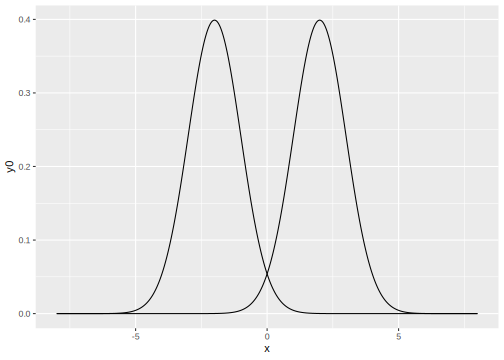
\includegraphics{design-notes_files/figure-latex/normals-same-var-1.pdf}
\caption{\label{fig:normals-same-var}Two normal variates with different means and same variance. Note this figure is a scalable vector graphic --- from what I understand, this is better from an accessbility standpoint.}
\end{figure}

The figure with caption caption is created by typing the code directly into the markdown document:

\begin{verbatim}
```{r normals-same-var, echo=TRUE, fig.cap="Two normal variates with different means and same variance. Note this figure is a scalable vector graphic --- from what I understand, this is better from an accessbility standpoint."}
  x <- seq(-8, 8, length=1000)
  y0 <- dnorm(x, -2, 1)
  y1 <- dnorm(x, 2, 1)
  df <- tibble(x, y0, y1)
  df <- melt(df, id.var = "x", value.name = "y")
  ggplot(data = df, aes(x = x, color = variable)) + geom_line(aes(y=y)) 
```
\end{verbatim}

\end{document}
